\documentclass[12pt]{article}
\usepackage{fullpage}

\usepackage[T1]{fontenc}
\usepackage[utf8]{inputenc}
\usepackage{lmodern}
\usepackage{microtype}
\usepackage{amsmath,amssymb,amsthm}
\usepackage{mathtools}
\usepackage{graphicx}
\usepackage{booktabs}
\usepackage{hyperref}
\usepackage{url}
\usepackage{xcolor}
\usepackage{enumitem}
\usepackage{amsfonts}
\usepackage{tikz}
\usetikzlibrary{arrows.meta,positioning,shapes.geometric,calc}

\hypersetup{colorlinks=true,linkcolor=blue,citecolor=blue,urlcolor=blue}

\theoremstyle{plain}
\newtheorem{theorem}{Theorem}
\newtheorem{proposition}[theorem]{Proposition}
\newtheorem{lemma}[theorem]{Lemma}
\newtheorem{corollary}[theorem]{Corollary}

\theoremstyle{definition}
\newtheorem{definition}[theorem]{Definition}

\theoremstyle{remark}
\newtheorem*{remark}{Remark}

\newcommand{\R}{\mathbb{R}}
\newcommand{\F}{\mathbf{F}}
\newcommand{\Gr}{\operatorname{Gr}}
\newcommand{\rank}{\operatorname{rank}}
\newcommand{\Seg}{\operatorname{Seg}}
\newcommand{\Pp}{\mathbb{P}}

\title{Solution to Problem 9 --- Quadrilinear Determinantal Tensors\\[6pt]
\large A submission to the First Proof challenge}

%% ====================================================================
%% AUTHOR: Replace the placeholder below with your name and details
%% ====================================================================
\author{
  Mark Dillerop\footnote{Email: dillerop@gmail.com}\\
  \textit{Independent / Ars Socratica}
}

\date{February 10, 2026}

\begin{document}
\maketitle

\begin{abstract}
We solve Problem~9 from the First Proof challenge \cite{FirstProof}.
Given $n \geq 5$ Zariski-generic matrices $A^{(1)}, \ldots, A^{(n)} \in \R^{3 \times 4}$ and the associated quadrilinear determinantal tensors $Q^{(\alpha\beta\gamma\delta)}$, we construct an explicit polynomial map $\F$ of degree~4 in the tensor entries, independent of the matrices and of $n$, that characterizes rank-1 scalings $\lambda_{\alpha\beta\gamma\delta} = u_\alpha v_\beta w_\gamma x_\delta$ on the non-identical support.
The map consists of six families of quartic Pl\"ucker-elimination equations, one per pair of tensor positions.
The answer is \textbf{YES}.
\end{abstract}

\tableofcontents
\newpage

%======================================================================
\section{Problem Statement}\label{sec:problem}
%======================================================================

The following is Problem~9 from the First Proof challenge \cite{FirstProof}, authored by Joe Kileel (University of Texas at Austin).

\medskip

Let $n \geq 5$.
Let $A^{(1)}, \ldots, A^{(n)} \in \R^{3 \times 4}$ be Zariski-generic.
For $\alpha, \beta, \gamma, \delta \in [n]$, construct $Q^{(\alpha \beta \gamma \delta)} \in \R^{3 \times 3 \times 3 \times 3}$ so that its $(i, j, k, \ell)$ entry for $1 \leq i, j, k, \ell \leq 3$ is given by
\[
Q^{(\alpha \beta \gamma \delta)}_{i j k \ell} = \det [A^{(\alpha)}(i, :);\; A^{(\beta)}(j, :);\; A^{(\gamma)}(k, :);\; A^{(\delta)}(\ell, :)].
\]
Here $A(i, :)$ denotes the $i$th row of a matrix $A$, and semicolon denotes vertical concatenation.
We are interested in algebraic relations on the set of tensors $\{Q^{(\alpha \beta \gamma \delta)} : \alpha, \beta, \gamma, \delta \in [n] \}$.

More precisely, does there exist a polynomial map $\F\colon \R^{81n^4} \rightarrow \R^N$ that satisfies the following three properties?
\begin{itemize}\setlength\itemsep{0.5em}
\item The map $\F$ does not depend on $A^{(1)}, \ldots, A^{(n)}$.
\item The degrees of the coordinate functions of $\F$ do not depend on $n$.
\item Let $\lambda \in \R^{n \times n \times n \times n}$ satisfy
$\lambda_{\alpha \beta \gamma \delta} \neq 0$ for precisely $\alpha, \beta, \gamma, \delta \in [n]$ that are not identical.  Then $\F(\lambda_{\alpha \beta \gamma \delta} Q^{(\alpha \beta \gamma \delta)} : \alpha, \beta, \gamma, \delta \in [n]) = 0$ holds if and only if there exist $u, v, w, x \in (\R^*)^n$ such that $\lambda_{\alpha \beta \gamma \delta} = u_{\alpha} v_{\beta} w_{\gamma} x_{\delta}$ for all $\alpha, \beta, \gamma, \delta \in [n]$ that are not identical.
\end{itemize}

%======================================================================
\section{Main Result}\label{sec:result}
%======================================================================

\begin{theorem}\label{thm:main}
Let $n \geq 5$. Let $A^{(1)}, \ldots, A^{(n)} \in \R^{3 \times 4}$ be Zariski-generic. Then there exists a polynomial map $\F\colon \R^{81n^4} \to \R^N$ such that:
\begin{enumerate}
\item $\F$ does not depend on $A^{(1)}, \ldots, A^{(n)}$.
\item The degrees of the coordinate functions of $\F$ are at most $4$. In particular, the degrees do not depend on $n$.
\item Let $\lambda_{\alpha\beta\gamma\delta} \neq 0$ for all non-identical $(\alpha,\beta,\gamma,\delta)$ (i.e., not all four equal). Then $\F(\lambda \cdot Q) = 0$ if and only if there exist $u, v, w, x \in (\R^*)^n$ with $\lambda_{\alpha\beta\gamma\delta} = u_\alpha v_\beta w_\gamma x_\delta$ for all non-identical $(\alpha,\beta,\gamma,\delta)$.
\end{enumerate}
\end{theorem}

\begin{remark}[Identical tuples]
The entries $\lambda_{\alpha\alpha\alpha\alpha}$ are unconstrained: since each $A^{(\alpha)} \in \R^{3 \times 4}$ has only $3$ rows, $Q^{(\alpha\alpha\alpha\alpha)}_{ijkl} = 0$ (repeated rows in a $4 \times 4$ matrix), so $T^{(\alpha\alpha\alpha\alpha)} \equiv 0$ regardless of $\lambda_{\alpha\alpha\alpha\alpha}$. No polynomial in $T$ that is independent of $A^{(1)}, \ldots, A^{(n)}$ can constrain these entries. The rank-1 characterization is therefore stated only on the non-identical support, which is the natural observable domain.
\end{remark}

\noindent\textbf{Answer: YES.}

%======================================================================
\section{Notation}\label{sec:notation}
%======================================================================

\begin{itemize}[nosep]
\item $a^{(\alpha)}_i \in \R^4$: $i$-th row of $A^{(\alpha)}$, for $i \in [3] := \{1,2,3\}$.
\item $Q^{(\alpha\beta\gamma\delta)}_{ijkl} = \det[a^{(\alpha)}_i;\, a^{(\beta)}_j;\, a^{(\gamma)}_k;\, a^{(\delta)}_l]$: quadrifocal tensor.
\item $T^{(\alpha\beta\gamma\delta)}_{ijkl} = \lambda_{\alpha\beta\gamma\delta} \cdot Q^{(\alpha\beta\gamma\delta)}_{ijkl}$: observed tensor.
\item Non-identical: not all four indices $\alpha,\beta,\gamma,\delta$ equal.
\item For $\{p,q\} \subset \{1,2,3,4\}$, write $\{r,s\} = \{1,2,3,4\} \setminus \{p,q\}$ for the complementary positions.
\end{itemize}

%======================================================================
\section{Idea of the Proof}\label{sec:idea}
%======================================================================

Each Pl\"ucker relation gives a quadratic identity among the $Q$-tensors. After scaling by $\lambda$, it becomes $P(I) = \mu \cdot S(I)$ where $\mu$ depends only on $\lambda$-ratios, not on row indices. Cross-multiplying two instances $I_1, I_2$ removes $\mu$ and yields quartic, polynomials in $T$ that are independent of $A^{(1)}, \ldots, A^{(n)}$. For generic matrices, these force vanishing of all $2 \times 2$ minors of certain $\lambda$-slices (pairwise rank-1 conditions). The six families---one per pair of positions---yield six such conditions, and a six-step algebraic peeling argument shows these jointly force $\lambda = u \otimes v \otimes w \otimes x$ on the non-identical support.

\begin{figure}[ht]
\centering
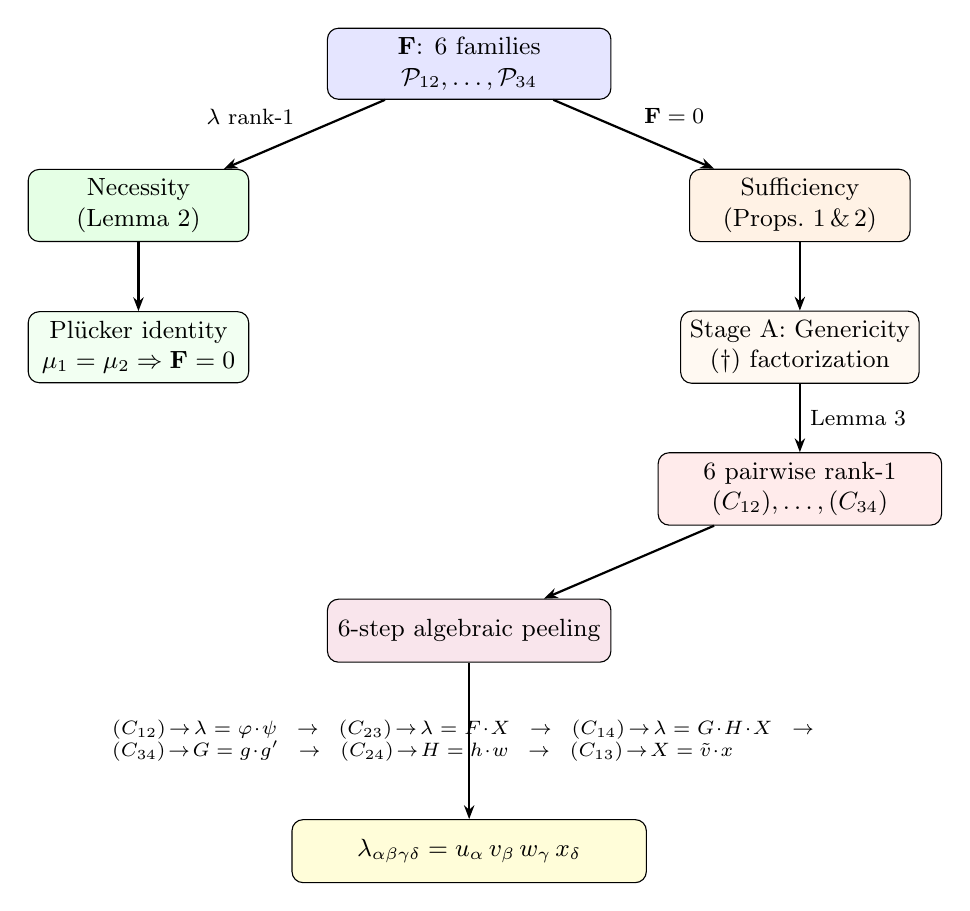
\begin{tikzpicture}[
  box/.style={draw, rounded corners, minimum width=2.8cm, minimum height=0.8cm, align=center, font=\small},
  bigbox/.style={draw, rounded corners, minimum width=3.6cm, minimum height=0.8cm, align=center, font=\small},
  arr/.style={-{Stealth[length=5pt]}, thick},
  every node/.style={font=\small}
]

% Top: Construction
\node[bigbox, fill=blue!10] (F) at (0,0) {$\mathbf{F}$: 6 families\\$\mathcal{P}_{12},\ldots,\mathcal{P}_{34}$};

% Necessity and Sufficiency branches
\node[box, fill=green!10] (nec) at (-4.2,-1.8) {Necessity\\(Lemma~2)};
\node[box, fill=orange!10] (suf) at (4.2,-1.8) {Sufficiency\\(Props.~1\,\&\,2)};

\draw[arr] (F) -- (nec) node[midway, above left, font=\footnotesize] {$\lambda$ rank-1};
\draw[arr] (F) -- (suf) node[midway, above right, font=\footnotesize] {$\mathbf{F}=0$};

% Necessity detail
\node[box, fill=green!5] (plucker) at (-4.2,-3.6) {Pl\"ucker identity\\$\mu_1 = \mu_2 \Rightarrow \mathbf{F}=0$};
\draw[arr] (nec) -- (plucker);

% Sufficiency Stage A
\node[box, fill=orange!5] (stageA) at (4.2,-3.6) {Stage A: Genericity\\$(\dagger)$ factorization};
\draw[arr] (suf) -- (stageA);

% Pairwise rank-1
\node[bigbox, fill=red!8] (pairwise) at (4.2,-5.4) {6 pairwise rank-1\\$(C_{12}),\ldots,(C_{34})$};
\draw[arr] (stageA) -- (pairwise) node[midway, right, font=\footnotesize] {Lemma~3};

% Stage B: 6-step peeling
\node[bigbox, fill=purple!10] (peeling) at (0,-7.2) {6-step algebraic peeling};
\draw[arr] (pairwise) -- (peeling);

% Steps
\node[font=\scriptsize, align=left, text width=9cm] (steps) at (0,-8.6) {%
$(C_{12})\!\to\!\lambda = \varphi\!\cdot\!\psi$ \;\;$\to$\;\;
$(C_{23})\!\to\!\lambda = F\!\cdot\!X$ \;\;$\to$\;\;
$(C_{14})\!\to\!\lambda = G\!\cdot\!H\!\cdot\!X$ \;\;$\to$\;\;
$(C_{34})\!\to\!G = g\!\cdot\!g'$ \;\;$\to$\;\;
$(C_{24})\!\to\!H = h\!\cdot\!w$ \;\;$\to$\;\;
$(C_{13})\!\to\!X = \tilde{v}\!\cdot\!x$};

% Conclusion
\node[bigbox, fill=yellow!15, minimum width=4.5cm] (conc) at (0,-10) {$\lambda_{\alpha\beta\gamma\delta} = u_\alpha\, v_\beta\, w_\gamma\, x_\delta$};
\draw[arr] (peeling) -- (conc);

\end{tikzpicture}
\caption{Structure of the proof. The polynomial map $\mathbf{F}$ (top) yields both necessity (left branch, via the Pl\"ucker identity) and sufficiency (right branch, via genericity and algebraic peeling).}
\label{fig:proof-structure}
\end{figure}

%======================================================================
\section{Construction of $\F$}\label{sec:construction}
%======================================================================

The map $\F$ consists of six families of Pl\"ucker equations, one for each pair of positions $\{p,q\} \subset \{1,2,3,4\}$.

Fix a pair $\{p,q\}$ with complement $\{r,s\}$ ($r < s$). For indices $c_p, c_q$ (shared) and $v_1, v_2, v_3, v_4$ (varying in positions $r, s$), define six 4-tuples by placing $c_p$ in position $p$, $c_q$ in position $q$, and the indicated indices in positions $r, s$:
\begin{align*}
\tau_1 &= (c_p, c_q;\, v_1, v_2), & \tau_2 &= (c_p, c_q;\, v_3, v_4), \\
\tau_3 &= (c_p, c_q;\, v_1, v_3), & \tau_4 &= (c_p, c_q;\, v_2, v_4), \\
\tau_5 &= (c_p, c_q;\, v_1, v_4), & \tau_6 &= (c_p, c_q;\, v_2, v_3),
\end{align*}
where $(c_p, c_q;\, v_r, v_s)$ denotes the 4-tuple with index $c_p$ in position $p$, $c_q$ in position $q$, $v_r$ in position $r$, $v_s$ in position $s$. Require all six 4-tuples to be non-identical.

For row-index 6-tuples $I_m = (i^m_p, i^m_q, i^m_1, i^m_2, i^m_3, i^m_4) \in [3]^6$ ($m = 1, 2$), the six components correspond to the row indices for $c_p, c_q, v_1, v_2, v_3, v_4$ respectively. Define:
\begin{align*}
P_{\{p,q\}}(I_m) &:= T^{\tau_1}_{(i^m_p, i^m_q, i^m_1, i^m_2)} \cdot T^{\tau_2}_{(i^m_p, i^m_q, i^m_3, i^m_4)}, \\[4pt]
S_{\{p,q\}}(I_m) &:= T^{\tau_3}_{(i^m_p, i^m_q, i^m_1, i^m_3)} \cdot T^{\tau_4}_{(i^m_p, i^m_q, i^m_2, i^m_4)} - T^{\tau_5}_{(i^m_p, i^m_q, i^m_1, i^m_4)} \cdot T^{\tau_6}_{(i^m_p, i^m_q, i^m_2, i^m_3)},
\end{align*}
where each subscript 4-tuple is ordered by position $(1,2,3,4)$, with the shared indices in positions $p,q$ and the varying indices in positions $r,s$. The equation is:
\begin{equation}\tag{$\mathcal{P}_{pq}$}
F^{\{p,q\}}_{(c_p,c_q,v_1,v_2,v_3,v_4),\,I_1,I_2} := P_{\{p,q\}}(I_1) \cdot S_{\{p,q\}}(I_2) - P_{\{p,q\}}(I_2) \cdot S_{\{p,q\}}(I_1).
\end{equation}
The map $\F$ is the collection of all $F^{\{p,q\}}$ equations over all six pairs $\{p,q\}$, all index choices, and all row-index pairs.

\medskip
\noindent\textbf{Explicit instantiation for $\{p,q\} = \{1,2\}$.}\quad Complement $\{r,s\} = \{3,4\}$. Shared indices $(c_1,c_2) = (\alpha,\beta)$. Varying indices $(v_1,v_2,v_3,v_4) = (\gamma,\delta,\gamma',\delta')$. Row indices $(i,j,k,l,k',l') \in [3]^6$. Then:
\begin{alignat*}{2}
\tau_1 &= (\alpha,\beta,\gamma,\delta), &\qquad J_1 &= (i,j,k,l), \\
\tau_2 &= (\alpha,\beta,\gamma',\delta'), &\qquad J_2 &= (i,j,k',l'), \\
\tau_3 &= (\alpha,\beta,\gamma,\gamma'), &\qquad J_3 &= (i,j,k,k'), \\
\tau_4 &= (\alpha,\beta,\delta,\delta'), &\qquad J_4 &= (i,j,l,l'), \\
\tau_5 &= (\alpha,\beta,\gamma,\delta'), &\qquad J_5 &= (i,j,k,l'), \\
\tau_6 &= (\alpha,\beta,\delta,\gamma'), &\qquad J_6 &= (i,j,l,k'),
\end{alignat*}
and $P(I) = T^{\tau_1}_{J_1} T^{\tau_2}_{J_2}$, \; $S(I) = T^{\tau_3}_{J_3} T^{\tau_4}_{J_4} - T^{\tau_5}_{J_5} T^{\tau_6}_{J_6}$.

\medskip
\noindent\textbf{Properties 1 and 2} are immediate: each $F^{\{p,q\}}$ is a degree-4 polynomial in the entries of $T$ only; no entry of $A^{(1)}, \ldots, A^{(n)}$ appears. The unknown ratio $\mu$ between $P(I)$ and $S(I)$ (see Section~\ref{sec:necessity}) is eliminated by cross-multiplying two instances $I_1, I_2$, ensuring $\F$ is polynomial (no denominators) and quartic in $T$.

%======================================================================
\section{Necessity ($\lambda$ rank-1 $\Rightarrow$ $\F = 0$)}\label{sec:necessity}
%======================================================================

\begin{lemma}[Pl\"ucker identity]\label{lem:plucker}
For any vectors $r_1, r_2, v_1, v_2, v_3, v_4 \in \R^4$:
\begin{multline*}
\det[r_1,r_2,v_1,v_2] \cdot \det[r_1,r_2,v_3,v_4] \\
= \det[r_1,r_2,v_1,v_3] \cdot \det[r_1,r_2,v_2,v_4] - \det[r_1,r_2,v_1,v_4] \cdot \det[r_1,r_2,v_2,v_3].
\end{multline*}
\end{lemma}

\begin{proof}
This is the Pl\"ucker relation for $\Gr(2,4)$; see \cite{KPRS06}, Eq.~(3), or equivalently \cite{GH78}, Ch.~1, \S5, eq.~(5.1), p.~211.
\end{proof}

\begin{lemma}\label{lem:necessity}
If $\lambda_{\alpha\beta\gamma\delta} = u_\alpha v_\beta w_\gamma x_\delta$, then $F^{\{p,q\}} = 0$ for all six pairs $\{p,q\}$.
\end{lemma}

\begin{proof}
We prove the case $\{p,q\} = \{1,2\}$; the other five follow by the same argument with the shared rows in positions $p,q$. (For $\{p,q\} \neq \{1,2\}$, reordering rows of the $4 \times 4$ determinant to place the shared rows first introduces a sign $(-1)^\sigma$ in each $Q$-factor, but these signs cancel in the degree-4 expression $F^{\{p,q\}}$ since each term is a product of two $Q$-factors sharing the same row permutation.)

With shared indices $(\alpha,\beta)$ in positions $(1,2)$ and varying indices $(\gamma,\delta,\gamma',\delta')$ in positions $(3,4)$, Lemma~\ref{lem:plucker} with $r_1 = a^{(\alpha)}_i$, $r_2 = a^{(\beta)}_j$ gives at the $Q$-level:
\[
Q^{(\alpha\beta\gamma\delta)}_{ijkl} \cdot Q^{(\alpha\beta\gamma'\delta')}_{ijk'l'} = Q^{(\alpha\beta\gamma\gamma')}_{ijkk'} \cdot Q^{(\alpha\beta\delta\delta')}_{ijll'} - Q^{(\alpha\beta\gamma\delta')}_{ijkl'} \cdot Q^{(\alpha\beta\delta\gamma')}_{ijlk'}.
\]
Substituting $T = \lambda \cdot Q$:
\[
P(I) = \lambda_{\alpha\beta\gamma\delta} \cdot \lambda_{\alpha\beta\gamma'\delta'} \cdot \bigl[Q^{(\alpha\beta\gamma\gamma')} Q^{(\alpha\beta\delta\delta')} - Q^{(\alpha\beta\gamma\delta')} Q^{(\alpha\beta\delta\gamma')}\bigr].
\]
For $S(I) = \lambda_{\alpha\beta\gamma\gamma'} \lambda_{\alpha\beta\delta\delta'} \cdot Q^{(\alpha\beta\gamma\gamma')} Q^{(\alpha\beta\delta\delta')} - \lambda_{\alpha\beta\gamma\delta'} \lambda_{\alpha\beta\delta\gamma'} \cdot Q^{(\alpha\beta\gamma\delta')} Q^{(\alpha\beta\delta\gamma')}$, the $\lambda$-ratios for rank-1 $\lambda$ are:
\[
\mu_1 := \frac{\lambda_{\alpha\beta\gamma\delta} \lambda_{\alpha\beta\gamma'\delta'}}{\lambda_{\alpha\beta\gamma\gamma'} \lambda_{\alpha\beta\delta\delta'}} = \frac{x_\delta w_{\gamma'}}{x_{\gamma'} w_\delta}, \qquad
\mu_2 := \frac{\lambda_{\alpha\beta\gamma\delta} \lambda_{\alpha\beta\gamma'\delta'}}{\lambda_{\alpha\beta\gamma\delta'} \lambda_{\alpha\beta\delta\gamma'}} = \frac{x_\delta w_{\gamma'}}{w_\delta x_{\gamma'}}.
\]
Since $\mu_1 = \mu_2 =: \mu$, we have $P(I) = \mu \cdot S(I)$ for all $I$. Therefore:
\[
F^{\{1,2\}} = P(I_1)\, S(I_2) - P(I_2)\, S(I_1) = \mu\, S(I_1)\, S(I_2) - \mu\, S(I_2)\, S(I_1) = 0. \qedhere
\]
\end{proof}

%======================================================================
\section{Sufficiency --- Pl\"ucker Equations Imply Pairwise Rank-1}\label{sec:suff1}
%======================================================================

\begin{proposition}\label{prop:pairwise}
For Zariski-generic $A^{(1)}, \ldots, A^{(n)}$, if $F^{\{p,q\}} = 0$ for all index and row-index choices, then for every pair $\{p,q\}$ and every choice of indices $c_p, c_q$, the matrix $M^{(c_p,c_q)}_{v_r, v_s} := \lambda_{(c_p, c_q;\, v_r, v_s)}$ has rank $1$ in $(v_r, v_s)$.
\end{proposition}

\begin{proof}
We prove the case $\{p,q\} = \{1,2\}$; the others follow by the same argument with positions relabeled.

\medskip\noindent\textbf{Factoring $F^{\{1,2\}}$.}\quad Write $\Lambda_P := \lambda_{\alpha\beta\gamma\delta} \lambda_{\alpha\beta\gamma'\delta'}$, \; $\Lambda_{S_1} := \lambda_{\alpha\beta\gamma\gamma'} \lambda_{\alpha\beta\delta\delta'}$, \; $\Lambda_{S_2} := \lambda_{\alpha\beta\gamma\delta'} \lambda_{\alpha\beta\delta\gamma'}$. Define:
\[
S_{Q,1}(I) := Q^{(\alpha\beta\gamma\gamma')}_{I_3} \cdot Q^{(\alpha\beta\delta\delta')}_{I_4}, \qquad S_{Q,2}(I) := Q^{(\alpha\beta\gamma\delta')}_{I_5} \cdot Q^{(\alpha\beta\delta\gamma')}_{I_6}.
\]
By Lemma~\ref{lem:plucker}, $P_Q(I) := Q^{(\alpha\beta\gamma\delta)}_{I_1} Q^{(\alpha\beta\gamma'\delta')}_{I_2} = S_{Q,1}(I) - S_{Q,2}(I)$. Then:
\[
P(I) = \Lambda_P \cdot [S_{Q,1}(I) - S_{Q,2}(I)], \qquad S(I) = \Lambda_{S_1} \cdot S_{Q,1}(I) - \Lambda_{S_2} \cdot S_{Q,2}(I).
\]
Expanding $F^{\{1,2\}} = P(I_1)\, S(I_2) - P(I_2)\, S(I_1)$:
\begin{equation}\tag{$\dagger$}\label{eq:dagger}
F^{\{1,2\}} = \Lambda_P \cdot (\Lambda_{S_1} - \Lambda_{S_2}) \cdot \bigl[S_{Q,1}(I_1) \cdot S_{Q,2}(I_2) - S_{Q,1}(I_2) \cdot S_{Q,2}(I_1)\bigr].
\end{equation}
\end{proof}

\begin{lemma}[Genericity]\label{lem:genericity}
For any $n \geq 5$ and any choice of indices $\gamma, \delta, \gamma', \delta'$ (with possible repetitions among $\alpha, \beta$), the bracket in \eqref{eq:dagger} is a polynomial in the entries of $A^{(1)}, \ldots, A^{(n)}$ that is not identically zero.
\end{lemma}

\begin{proof}
It suffices to exhibit one configuration where the bracket is nonzero (since a polynomial that is nonzero at a point is nonzero on a Zariski-open dense set). Consider matrices $A^{(m)}$ with rows
\[
a^{(m)}_1 = (1,0,0,m), \quad a^{(m)}_2 = (0,1,0,m^2), \quad a^{(m)}_3 = (0,0,1,m^3)
\]
for $m = 1, \ldots, n$. Take $\alpha = 1, \beta = 2$ (shared), $\gamma = 3, \delta = 4, \gamma' = 5, \delta' = 6$ (or $\delta' = 1$ if $n = 5$). Choose $I_1 = (1,1,2,2,3,3)$ and $I_2 = (1,1,2,3,2,3)$.

\smallskip\noindent\emph{For $I_1$:} the shared rows are $a^{(1)}_1 = (1,0,0,1)$ and $a^{(2)}_1 = (1,0,0,2)$, with varying rows of type $a^{(\cdot)}_2 = (0,1,0,\cdot)$ and $a^{(\cdot)}_3 = (0,0,1,\cdot)$. By cofactor expansion along the first two rows (which differ only in the last entry), every determinant of the form $\det[a^{(1)}_1, a^{(2)}_1, a^{(\cdot)}_2, a^{(\cdot)}_3]$ equals $t_\beta - t_\alpha = 1$, independent of the varying matrices. Therefore $S_{Q,1}(I_1) = 1$ and $S_{Q,2}(I_1) = 1$.

\smallskip\noindent\emph{For $I_2$:} the varying rows are $(2,3,2,3)$ instead of $(2,2,3,3)$. The factors of $S_{Q,1}(I_2)$ involve determinants $\det[a^{(1)}_1, a^{(2)}_1, a^{(\gamma)}_2, a^{(\gamma')}_2]$ and $\det[a^{(1)}_1, a^{(2)}_1, a^{(\delta)}_3, a^{(\delta')}_3]$. Each has two rows of the form $(0,1,0,\cdot)$ or $(0,0,1,\cdot)$, giving a $4 \times 4$ matrix with rank $\leq 3$. Hence both determinants are $0$, so $S_{Q,1}(I_2) = 0$.

The factor $S_{Q,2}(I_2)$ involves $\det[a^{(1)}_1, a^{(2)}_1, a^{(\gamma)}_2, a^{(\delta')}_3] \cdot \det[a^{(1)}_1, a^{(2)}_1, a^{(\delta)}_3, a^{(\gamma')}_2]$. The first determinant equals $1$ (same structure as $I_1$). The second has rows $a^{(\cdot)}_3$ before $a^{(\cdot)}_2$ in positions 3,4, giving $-1$ (one row swap). So $S_{Q,2}(I_2) = -1$.

Therefore the bracket equals $1 \cdot (-1) - 0 \cdot 1 = -1 \neq 0$. The same computation applies for $n = 5$ with $\delta' = \alpha$ (repeated index), since the determinant structure depends only on the row types.
\end{proof}

\medskip
\noindent\emph{Proof of Proposition~\ref{prop:pairwise} (continued).}\quad Since the bracket is a nonzero polynomial, it is nonzero on a Zariski-open dense subset of the parameter space of $(A^{(1)}, \ldots, A^{(n)})$. Combined with $\Lambda_P \neq 0$ (all $\lambda$-values on non-identical tuples are nonzero), we conclude from \eqref{eq:dagger}:
\begin{equation}\tag{$C_{12}$}\label{eq:star12}
\Lambda_{S_1} = \Lambda_{S_2}, \quad \text{i.e.,} \quad \lambda_{\alpha\beta\gamma\gamma'} \lambda_{\alpha\beta\delta\delta'} = \lambda_{\alpha\beta\gamma\delta'} \lambda_{\alpha\beta\delta\gamma'}.
\end{equation}
This is the vanishing of all $2 \times 2$ minors of $M^{(\alpha,\beta)}_{\gamma,\delta} = \lambda_{\alpha\beta\gamma\delta}$, i.e., $\rank M^{(\alpha,\beta)} = 1$. \qed

\medskip
Applying Proposition~\ref{prop:pairwise} to all six pairs yields six pairwise rank-1 conditions:
\begin{itemize}[nosep]
\item $(C_{12})$: For fixed $(\alpha,\beta)$, $\lambda_{\alpha\beta\gamma\delta}$ is rank-1 in $(\gamma,\delta)$.
\item $(C_{13})$: For fixed $(\alpha,\gamma)$, $\lambda_{\alpha\beta\gamma\delta}$ is rank-1 in $(\beta,\delta)$.
\item $(C_{14})$: For fixed $(\alpha,\delta)$, $\lambda_{\alpha\beta\gamma\delta}$ is rank-1 in $(\beta,\gamma)$.
\item $(C_{23})$: For fixed $(\beta,\gamma)$, $\lambda_{\alpha\beta\gamma\delta}$ is rank-1 in $(\alpha,\delta)$.
\item $(C_{24})$: For fixed $(\beta,\delta)$, $\lambda_{\alpha\beta\gamma\delta}$ is rank-1 in $(\alpha,\gamma)$.
\item $(C_{34})$: For fixed $(\gamma,\delta)$, $\lambda_{\alpha\beta\gamma\delta}$ is rank-1 in $(\alpha,\beta)$.
\end{itemize}

%======================================================================
\section{Sufficiency --- Pairwise Rank-1 Implies Rank-1}\label{sec:suff2}
%======================================================================

\begin{proposition}\label{prop:rank1}
If $\lambda_{\alpha\beta\gamma\delta} \neq 0$ for all non-identical $(\alpha,\beta,\gamma,\delta)$ and the six conditions $(C_{12})$--$(C_{34})$ hold, then there exist $u, v, w, x \in (\R^*)^n$ such that $\lambda_{\alpha\beta\gamma\delta} = u_\alpha v_\beta w_\gamma x_\delta$ for all non-identical $(\alpha,\beta,\gamma,\delta)$.
\end{proposition}

\begin{proof}
We extract the rank-1 factorization in six steps, each using one pairwise condition. Fix five distinct reference indices $a_0, b_0, c_0, d_0, e_0 \in [n]$ (possible since $n \geq 5$).

\medskip\noindent\textbf{Step 1.}\quad By $(C_{12})$, for each fixed $(\alpha,\beta)$, the matrix $\lambda_{\alpha\beta\gamma\delta}$ has rank~1 in $(\gamma,\delta)$ on non-identical tuples. So:
\[
\lambda_{\alpha\beta\gamma\delta} = \varphi(\alpha,\beta,\gamma) \cdot \psi(\alpha,\beta,\delta)
\]
for all non-identical $(\alpha,\beta,\gamma,\delta)$. Explicitly: for each $(\alpha,\beta)$, choose a pivot $c_*(\alpha,\beta) \in \{c_0, e_0\}$ such that $c_* \neq \alpha$ (possible since $c_0 \neq e_0$). Then $(\alpha,\beta,c_*,\delta)$ is non-identical for all $\delta$ (since $c_* \neq \alpha$), so we may define:
\[
\psi(\alpha,\beta,\delta) := \lambda_{\alpha\beta\, c_*\, \delta}, \qquad \varphi(\alpha,\beta,\gamma) := \frac{\lambda_{\alpha\beta\gamma d_0}}{\psi(\alpha,\beta,d_0)}.
\]
All evaluations are at non-identical tuples (since $c_* \neq \alpha$ and $d_0 \notin \{c_0, e_0\}$ can be chosen distinct from $c_*$).

\medskip\noindent\textbf{Step 2.}\quad By $(C_{23})$, for each fixed $(\beta,\gamma)$, $\lambda_{\alpha\beta\gamma\delta}$ is rank-1 in $(\alpha,\delta)$. Substituting Step~1: $\varphi(\alpha,\beta,\gamma) \cdot \psi(\alpha,\beta,\delta)$ must be rank-1 in $(\alpha,\delta)$ for fixed $(\beta,\gamma)$. The $\varphi$-factors cancel (nonzero), leaving:
\[
\psi(\alpha_1,\beta,\delta_1)\, \psi(\alpha_2,\beta,\delta_2) = \psi(\alpha_1,\beta,\delta_2)\, \psi(\alpha_2,\beta,\delta_1).
\]
So for fixed $\beta$, $\psi(\alpha,\beta,\delta)$ is rank-1 in $(\alpha,\delta)$: $\psi(\alpha,\beta,\delta) = \psi_0(\alpha,\beta) \cdot X(\beta,\delta)$, where $X(\beta,\delta) := \psi(a_0,\beta,\delta)/\psi(a_0,\beta,d_0)$ and $\psi_0(\alpha,\beta) := \psi(\alpha,\beta,d_0)$.

Substituting: $\lambda_{\alpha\beta\gamma\delta} = F(\alpha,\beta,\gamma) \cdot X(\beta,\delta)$, where $F := \varphi \cdot \psi_0$.

\medskip\noindent\textbf{Step 3.}\quad By $(C_{14})$, for fixed $(\alpha,\delta)$, $\lambda$ is rank-1 in $(\beta,\gamma)$. The $X$-factors cancel in the $2 \times 2$ minor, so $F$ is rank-1 in $(\beta,\gamma)$ for fixed $\alpha$:
\[
F(\alpha,\beta,\gamma) = G(\alpha,\beta) \cdot H(\alpha,\gamma).
\]
Therefore $\lambda_{\alpha\beta\gamma\delta} = G(\alpha,\beta) \cdot H(\alpha,\gamma) \cdot X(\beta,\delta)$.

\medskip\noindent\textbf{Step 4.}\quad By $(C_{34})$, for fixed $(\gamma,\delta)$, $\lambda$ is rank-1 in $(\alpha,\beta)$. The $H$ and $X$ factors cancel: $G(\alpha_1,\beta_1)\, G(\alpha_2,\beta_2) = G(\alpha_1,\beta_2)\, G(\alpha_2,\beta_1)$. So $G$ is rank-1:
\[
G(\alpha,\beta) = g(\alpha) \cdot g'(\beta).
\]
Therefore $\lambda_{\alpha\beta\gamma\delta} = g(\alpha) \cdot g'(\beta) \cdot H(\alpha,\gamma) \cdot X(\beta,\delta)$.

\medskip\noindent\textbf{Step 5.}\quad By $(C_{24})$, for fixed $(\beta,\delta)$, $\lambda$ is rank-1 in $(\alpha,\gamma)$. The bracket $g'(\beta)\, X(\beta,\delta)$ is a scalar, so $g(\alpha)\, H(\alpha,\gamma)$ must be rank-1 in $(\alpha,\gamma)$. The $g$-factors cancel, so $H$ is rank-1:
\[
H(\alpha,\gamma) = h(\alpha) \cdot w(\gamma).
\]
Therefore $\lambda_{\alpha\beta\gamma\delta} = g(\alpha)\, h(\alpha) \cdot g'(\beta) \cdot w(\gamma) \cdot X(\beta,\delta)$.

\medskip\noindent\textbf{Step 6.}\quad By $(C_{13})$, for fixed $(\alpha,\gamma)$, $\lambda$ is rank-1 in $(\beta,\delta)$. The bracket $g(\alpha)\, h(\alpha)\, w(\gamma)$ is a scalar, so $g'(\beta)\, X(\beta,\delta)$ must be rank-1 in $(\beta,\delta)$. The $g'$-factors cancel, so $X$ is rank-1:
\[
X(\beta,\delta) = \tilde{v}(\beta) \cdot x(\delta).
\]

\medskip\noindent\textbf{Conclusion.}\quad Setting $u(\alpha) := g(\alpha)\, h(\alpha)$, $v(\beta) := g'(\beta)\, \tilde{v}(\beta)$:
\[
\lambda_{\alpha\beta\gamma\delta} = u(\alpha) \cdot v(\beta) \cdot w(\gamma) \cdot x(\delta)
\]
for all non-identical $(\alpha,\beta,\gamma,\delta)$. All factors are nonzero since $\lambda \neq 0$ on non-identical tuples.
\end{proof}

\begin{remark}
The rank-1 tensors form the Segre variety $\Seg(\Pp^{n-1} \times \Pp^{n-1} \times \Pp^{n-1} \times \Pp^{n-1})$, cut out by $2 \times 2$ minors of all mode flattenings \cite{Ha02}, Corollary~1.6.1. Proposition~\ref{prop:rank1} shows that the six pairwise rank-1 conditions $(C_{12})$--$(C_{34})$---which are precisely the $2 \times 2$ minors of the six $\binom{4}{2}$ flattenings---suffice to place $\lambda$ on the Segre variety (restricted to the non-identical support).
\end{remark}

%======================================================================
\section{Summary}\label{sec:summary}
%======================================================================

The polynomial map $\F$ consists of six families of quartic Pl\"ucker-elimination equations $\mathcal{P}_{12}, \mathcal{P}_{13}, \mathcal{P}_{14}, \mathcal{P}_{23}, \mathcal{P}_{24}, \mathcal{P}_{34}$, totaling $O(n^6 \cdot 3^{12})$ equations. The proof establishes:
\begin{enumerate}
\item \textbf{Independence from $A^{(1)}, \ldots, A^{(n)}$}: $\F$ is expressed purely in terms of $T$-entries.
\item \textbf{Bounded degree}: all coordinate functions have degree~4, independent of $n$.
\item \textbf{Exact characterization} (for Zariski-generic $A^{(1)}, \ldots, A^{(n)}$): $\F(\lambda \cdot Q) = 0 \iff \lambda$ is rank-1 on the non-identical support.
\end{enumerate}

The assumption $n \geq 5$ is used in two places: (i)~the Pl\"ucker equations require six index slots (two shared, four varying), and for $n = 5$ some varying indices must repeat a shared index---this is valid since the problem defines $\lambda_{\alpha\beta\gamma\delta} \neq 0$ for non-identical (not all-same) tuples, so e.g.\ $(\alpha,\beta,\gamma,\alpha)$ is permitted; (ii)~the factor extraction in Proposition~\ref{prop:rank1} requires five distinct reference indices $a_0, b_0, c_0, d_0, e_0$. The genericity witness in Lemma~\ref{lem:genericity} applies equally to $n = 5$ (with $v_4 = c_p$), as verified by explicit computation.\footnote{In the computer vision literature, the matrices $A^{(\alpha)}$ are called \emph{camera matrices} and the tensors $Q^{(\alpha\beta\gamma\delta)}$ are called \emph{quadrifocal tensors}. We use the problem's original terminology throughout.} For $n \leq 4$, the problem is open under this proof technique. \qed

%======================================================================
\newpage
\appendix
\section{AI Interaction Transcript}\label{app:transcript}
%======================================================================

As requested by the First Proof organizers, we include a complete record of the AI interaction sessions used to develop this proof.

\medskip\noindent\textbf{Timeline:} February 10, 2026, approximately 05:45--18:00 CET. Six sessions in one day, approximately 4--5 hours of active working time.\\
\textbf{AI systems used:} Claude Opus 4.6 (Anthropic), ChatGPT 5.2 Pro and ChatGPT 5.2 (OpenAI), Gemini 3 (Google). Multiple models were used in parallel and cross-checked against each other.\\
\textbf{Numerical verification:} Python/NumPy scripts generated by the AI and executed locally (no symbolic algebra systems).\\
\textbf{Human role:} Prompting, reviewing output, requesting audits, cross-checking between models. No mathematical ideas or content were provided by the human operator.

\subsection*{Example Prompts}

The following are representative prompts used during the sessions:

\begin{enumerate}[nosep]
\item \textit{``Help me to tackle this problem statement. It is part of First Proof. What are options to tackle this, which would you recommend and why?''}
\item \textit{``What are gaps to be filled? How solid is your suggested proof? Of the three proposed options, go through them one by one to see where they hold, where they break, and why.''}
\item \textit{``How well does the proof meet the criteria as set forward by First Proof?''}
\item \textit{``I had the previous proof reviewed by ChatGPT 5.2 Pro:''} [followed by 9-point detailed feedback on identical tuples, pivot safety, $n \geq 5$ justification, notation, and exposition]
\item \textit{``Should it be converted to a tex file pdf?''}
\end{enumerate}

\subsection*{Session 1 --- Kickoff \normalfont\textit{[Claude Opus 4.6]}}

\begin{itemize}[nosep]
\item Read problem statement. Clarified that ``non-identical'' means not all four indices equal (repeated indices allowed).
\item Populated references with 12 key papers: Hartley--Zisserman (quadrifocal tensor), Heyden (algebraic varieties), Alzati--Tortora (tensor rank), Landsberg (tensor geometry), etc.
\item Identified two candidate families of polynomial equations:
  \begin{itemize}[nosep]
  \item \textbf{Family A (degree 2):} Swap equations from transposition symmetry of rank-1 tensors.
  \item \textbf{Family B (degree 4):} Pl\"ucker relations from the Grassmannian structure.
  \end{itemize}
\end{itemize}

\subsection*{Session 2 --- Numerical verification \normalfont\textit{[Claude Opus 4.6, ChatGPT 5.2]}}

\begin{itemize}[nosep]
\item Generated Python verification scripts using NumPy.
\item Verified Family B (Pl\"ucker equations) for $n=5$ (with repeated indices) and $n=8$ (distinct indices). Both pass for rank-1 $\lambda$, fail for random $\lambda$.
\item Verified Family A (swap equations). Discovered a subtlety: the two 4-tuples must share indices in the swapped positions.
\item Wrote initial drafts of approach and proof documents.
\end{itemize}

\subsection*{Session 3 --- Corrected proof \normalfont\textit{[Claude Opus 4.6]}}

\begin{itemize}[nosep]
\item Re-verified corrected swap equations numerically: all 6 transpositions pass for rank-1 $\lambda$ (error $\sim 10^{-16}$), fail for random $\lambda$ (error $\sim 2.0$).
\item Rewrote proof with corrected swap equation definition.
\item Updated sufficiency argument: swap equations give $\lambda = h(\text{multiset}) \cdot u_\alpha v_\beta w_\gamma x_\delta$.
\end{itemize}

\subsection*{Session 4 --- Fundamental correction \normalfont\textit{[Claude Opus 4.6, Gemini 3]}}

\begin{itemize}[nosep]
\item \textbf{Critical discovery:} Step~1 of the sufficiency proof (swap equations $\to$ $h(\text{multiset}) \cdot uvwx$) was \textbf{wrong}. Numerical verification showed cross-cocycle consistency fails (error $\sim 1.93$).
\item \textbf{Breakthrough:} Discovered that 6 families of Pl\"ucker equations (one per pair $\{p,q\} \subset \{1,2,3,4\}$) suffice---no swap equations needed.
\item Developed the factorization $F^{\{p,q\}} = \Lambda_P \cdot (\Lambda_{S_1} - \Lambda_{S_2}) \cdot [\text{Q-bracket}]$.
\item Proved the 6-step algebraic peeling argument: pairwise rank-1 $\Rightarrow$ rank-1.
\item All 6 steps verified numerically (reconstruction error $\sim 10^{-15}$).
\item All 6 Pl\"ucker families verified for $n=5$ and $n=6$.
\end{itemize}

\subsection*{Session 5 --- Hardening \normalfont\textit{[Claude Opus 4.6]}}

\begin{itemize}[nosep]
\item Performed rigorous audit. Identified 1 critical issue, 3 medium, 2 low.
\item \textbf{C1 FIXED (critical):} Genericity argument was hand-wavy. Added Lemma~\ref{lem:genericity} with explicit witness matrices $A^{(m)}$ with rows $(1,0,0,m)$, $(0,1,0,m^2)$, $(0,0,1,m^3)$. Bracket $= -1 \neq 0$.
\item \textbf{M1 FIXED:} Row-reordering signs for non-$\{1,2\}$ pairs (signs cancel in degree-4 expression).
\item \textbf{M2 FIXED:} Row-index notation clarified with explicit subscript 4-tuples.
\item \textbf{M3 FIXED:} Genericity witness verified for $n=5$ with repeated indices.
\item Fixed 0-indexed vs 1-indexed row inconsistency.
\end{itemize}

\subsection*{Session 6 --- Publication preparation \normalfont\textit{[ChatGPT 5.2 Pro, Claude Opus 4.6]}}

\begin{itemize}[nosep]
\item Created self-contained submission file.
\item Cross-checked the proof using ChatGPT 5.2 Pro as an independent reviewer, which identified 9 points for improvement:
  \begin{itemize}[nosep]
  \item Clarified rank-1 definition for identical tuples ($\lambda_{\alpha\alpha\alpha\alpha}$ unobservable).
  \item Added explicit worked example for $\{p,q\} = \{1,2\}$ with $\tau_m$ and $J_m$ table.
  \item Added ``no divisions'' explanation for polynomiality.
  \item Fixed pivot construction to avoid $\lambda_{\alpha\alpha\alpha\alpha}$ ($c_*$ pivot with 5th reference index).
  \item Corrected $n \geq 5$ paragraph with precise justification.
  \item Added ``Idea of the proof'' section.
  \item Added Segre variety remark.
  \end{itemize}
\item All fixes implemented using Claude Opus 4.6. Converted to \LaTeX\ and compiled to PDF.
\end{itemize}

\subsection*{Summary of AI Contributions}

\begin{enumerate}[nosep]
\item \textbf{Literature survey:} Identified relevant references on quadrifocal tensors, tensor rank, and Grassmannian geometry.
\item \textbf{Equation discovery:} Identified the Pl\"ucker families and their correct formulations through algebraic analysis and numerical experimentation.
\item \textbf{Numerical verification:} Python scripts confirming equations hold for rank-1 $\lambda$ and fail for generic $\lambda$, for $n=5$ and $n=6$.
\item \textbf{Bug finding (Session 2):} Discovered and corrected the swap equation formulation through numerical falsification.
\item \textbf{Fundamental correction (Session 4):} Discovered that swap equations alone are insufficient. Replaced with 6 Pl\"ucker families and a clean 6-step algebraic argument.
\item \textbf{Proof writing:} Two-stage sufficiency argument (Pl\"ucker $\to$ pairwise rank-1 $\to$ rank-1 via 6-step peeling).
\end{enumerate}

%======================================================================
\begin{thebibliography}{99}
%======================================================================

\bibitem{FirstProof}
M.~Abouzaid, A.J.~Blumberg, M.~Hairer, J.~Kileel, T.G.~Kolda, P.D.~Nelson, D.~Spielman, N.~Srivastava, R.~Ward, S.~Weinberger, L.~Williams,
``First Proof,''
arXiv:2602.05192, 2026.

\bibitem{KPRS06}
R.~Kasman, K.~Pedings, A.~Reisz, T.~Shiota,
``Universality of rank-6 Pl\"ucker relations and Grassmann cone preserving maps,''
\emph{Proc.\ Amer.\ Math.\ Soc.} \textbf{136}(1), 77--87, 2008.
arXiv:math/0510093.
Eq.~(3): the 3-term Pl\"ucker relation for $\Gr(2,n)$.

\bibitem{GH78}
P.~Griffiths, J.~Harris,
\emph{Principles of Algebraic Geometry},
Wiley-Interscience, 1978.
Ch.~1, \S5, eq.~(5.1), p.~211.

\bibitem{Ha02}
H.T.~Ha,
``Box-shaped matrices and the defining ideal of certain blowup surfaces,''
\emph{J.\ Pure Appl.\ Algebra} \textbf{167}(2--3), 203--224, 2002.
arXiv:math/0210251.
Corollary~1.6.1: $I_2(A)$ is the defining ideal of the Segre embedding.

\end{thebibliography}

\end{document}
